% asset_id: FAS2GeometricDistributionTikZ-003 optional
\documentclass[tikz,border=8pt]{standalone}
\usepackage{amsmath}
\begin{document}
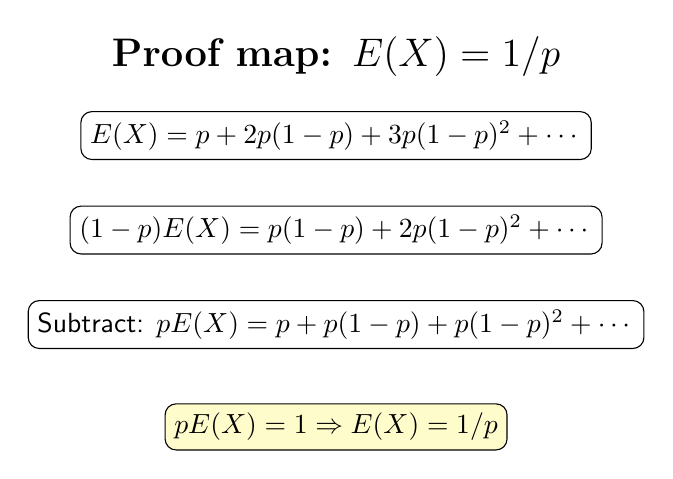
\begin{tikzpicture}[font=\sffamily]
\node[font=\bfseries\Large] at (6,3) {Proof map: $E(X)=1/p$};
\node[draw,rounded corners,align=left] at (6,2) {$E(X)=p+2p(1-p)+3p(1-p)^2+\cdots$};
\node[draw,rounded corners,align=left] at (6,.8) {$(1-p)E(X)=p(1-p)+2p(1-p)^2+\cdots$};
\node[draw,rounded corners,align=left] at (6,-.4) {Subtract: $pE(X)=p+p(1-p)+p(1-p)^2+\cdots$};
\node[draw,rounded corners,fill=yellow!20] at (6,-1.7) {$pE(X)=1\Rightarrow E(X)=1/p$};
\end{tikzpicture}\end{document}
